\section{Preprocessing}
To enable a machine learning model to process textual data effectively, it is essential to convert the text into numerical representations. The first step in this process is tokenizing the text, which involves splitting sentences into smaller units, such as words. For this task, we utilize a custom RegexpTokenizer from the NLTK library, which filters the text to retain only words, numbers, and a limited set of special characters. This ensures that irrelevant symbols are excluded while preserving the meaningful components of the text.

Following tokenization, the text is further refined by removing stopwords and applying stemming. Stopwords, which are frequently used words such as "the," "is," and "and," are removed as they are unlikely to contribute significant value to sentiment analysis. This is particularly important when using a limited sequence length for input sentences, as it allows the model to focus on more informative features while reducing the size of the vocabulary. Consequently, the model learns fewer parameters, which can improve its generalization and efficiency.

In addition, we apply stemming using the PorterStemmer from the NLTK library, which reduces words to their base or root forms (e.g., "feeling" becomes "feel"). This process further reduces the vocabulary size by grouping inflected or derived word forms together, helping the model to recognize similar meanings and improve its performance.

To better understand the text data after preprocessing, we visualize the most common words using a WordCloud, as shown in Figure \ref{fig:wordcloud}. This provides an intuitive way to analyze the prominent terms in the dataset and assess whether the preprocessing aligns with the goals of the sentiment analysis task.
\begin{figure}[H]
    \vspace*{0.7cm}
    \centering
    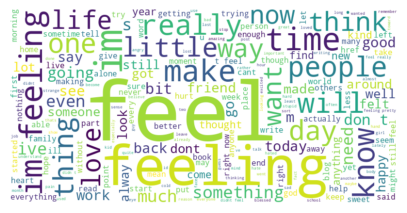
\includegraphics[width=0.4\textwidth]{figures/wordcloud.png}
    \caption{WordCloud of the vocabulary.}
    \label{fig:wordcloud}
    \vspace*{0.7cm}
\end{figure}
As expected many emotional words are present in the vocabulary, e.g. 'love', 'friend', 'hate', 'never', 'go', etc.

To be able to process the text data, we need to choose a maximum sentence length. A boxplot of the distribution of the lengths of the sequences can be seen in Figure \ref{fig:sequence_length}.
\begin{figure}[H]
    \vspace*{0.7cm}
    \centering
    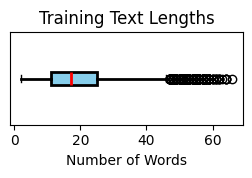
\includegraphics[width=0.22\textwidth]{figures/sentence_length.png}
    \caption{Distribution of the lengths of the sequences.}
    \label{fig:sequence_length}
    \vspace*{0.7cm}
\end{figure}
From the boxplot, we see that the majority of the sequences have a length of around 8 words. We choose to set the maximum sequence length to 10 words. This means that all sequences longer than 10 words are truncated, and all sequences shorter than 23 words are padded with a special token, '<PAD>', to make them all the same length. In addition, we discovered that some sentences are very short, therefore we choose to remove all sentences with a length less than 3 words.

Having our cleaned and tokenized text data, we build a vocabulary from the training dataset. The vocabulary is built by mapping each unique word to an integer. The vocabulary for the training dataset ended up being 10,336 words.

Then, we convert the text data to integers by mapping each word in the text data to the corresponding integer in the vocabulary and pad the sequences to the maximum sequence length. This is done for both the training, validation and test datasets. The text data is now ready to be used for a model.